% !TeX spellcheck = pl_PL

\chapter{Implementacja systemu uwierzytelniania}
\label{chp:implementation}
W tym rozdziale przedstawiam system uwierzytelniania wykorzystujący $NDB$ jako formę składowania skrótu hasła. 
Aplikacja nie przechowuje żadnych dodatkowych danych użytkownika, lecz może posłużyć jako baza dla systemów o~dokładniej sprecyzowanym zastosowaniu.

Implementacja jest napisana w języku C++17 z~użyciem biblioteki Qt, pozwalającej na łatwe projektowanie interfejsu użytkownika oraz dostarczającej
wszystkie wymagane procedury kryptograficzne.
\section{Reprezentacja danych}
Część danych użytkownika pozwalających na zalogowanie się do systemu znajdują się w zwykłej, relacyjnej bazie danych.
W tym celu została użyta baza SQLite3, oferująca możliwość szybkiego wdrożenia bez konieczności złożonej konfiguracji systemu.
W razie potrzeby przechowywania danych wielu klientów istnieje możliwość zamiany silnika bazy danych na bardziej 
zoptymalizowany pod kątem przechowywania wielu rekordów oraz obsługujący większą liczbę zapytań w jednym czasie.


\begin{figure}[h]
    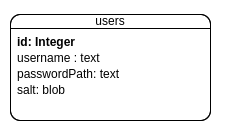
\includegraphics{img/diagrams/erd.png}
    \centering
    \caption{Diagram ERD aplikacji}
    \label{img:erd}
\end{figure}

System w formie bazowej używa tylko jednej tabeli -- \textit{users}, przechowującej:
\begin{itemize}
    \item id -- unikalny identyfikator rekordu
    \item username -- nazwa użytkownika, używana do logowania
    \item passwordPath -- ścieżka do pliku zawierającego formułę $NDB$ kodującą skrót hasła
    \item salt -- \enquote{sól} -- parametr algorytmu uzyskiwania klucza na podstawie frazy hasłowej
\end{itemize}
W przypadku potrzeby przechowywania dodatkowych danych należy dodać do tej tabeli klucze obce łączące użytkowników z~pozostałymi obiektami pozytywnej bazy danych.

W trakcie procedury tworzenia użytkownika generowany jest skrót hasła za pomocą algorytmu PBKDF2 z~użyciem funkcji skrótu SHA-512 oraz losowej soli.
Metoda jest ustawiona na 10000 iteracji i~generuje skrót o~długości 512 bitów. 
Do generacji $NDB$ używany jest algorytm \textit{K-Hidden}, który został wyłoniony na podstawie testów jako najbardziej bezpieczny.
Ponieważ jest to niekompletna metoda generacji konieczne jest zawarcie sumy kontrolnej -- do tego ponownie używana jest funkcja skrótu SHA-512.
Finalny rekord pozytywny jest konkatenacją wyniku funkcji PBKDF2 oraz sumy kontrolnej i~jego długość wynosi 1024 bity.

Tak skonstruowany ciąg bitowy jest kodowany do postaci negatywnej wykorzystując parametry przy których czas rozwiązywania okazał się najdłuższy tj. $p = \{0.7, 0, 0.3\}$, $k = 3$ i~$r = 4.5$.
Następnie powstała $NDB$ jest zapisywana do pliku w formacie \textit{ndb} (zbiór napisów na alfabetem $\{0,1,*\}$), którego ścieżka jest zapisana w kolumnie \textit{passwordPath}. 

\section{Działanie aplikacji}

Aplikacja posiada prosty graficzny interfejs użytkownika składający się z~trzech widoków - logowania, rejestracji oraz panelu użytkownika. Po uruchomieniu widoczne jest okno logowania. Z~tego poziomu można wpisać login i~hasło 
-- jeśli system uzna je za poprawne, to następuje przekierowanie do widoku użytkownika. 

\begin{figure}[h]
    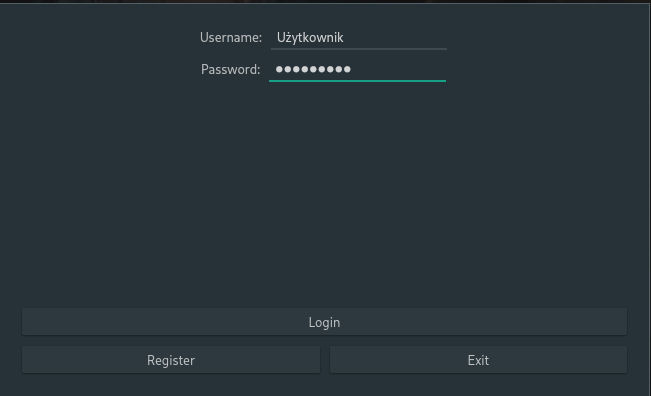
\includegraphics[width=10cm]{img/UI/login.png}
    \centering
    \caption{Panel logowania}
    \label{img:gui-login}
\end{figure}

Po kliknięciu przycisku \textit{Register} na panelu logowania pojawia się widok rejestracji. Tutaj można wprowadzić nowe dane uwierzytelniania i~potwierdzić je ponownie naciskając przycisk \textit{Register} -- jeśli hasło spełnia wymagania,
następuje powrót do widoku loginu, gdzie można uwierzytelnić się nowymi danymi.

\begin{figure}[h]
    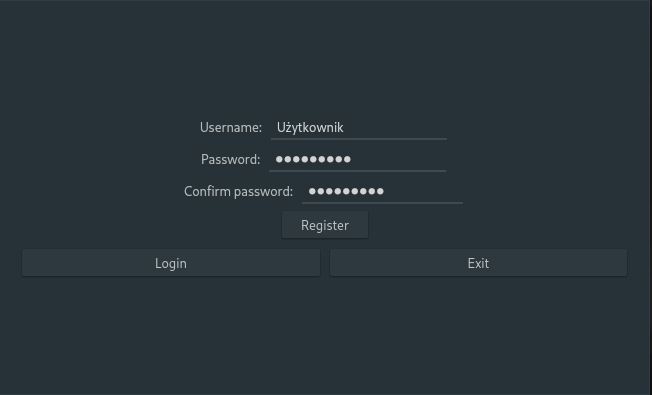
\includegraphics[width=10cm]{img/UI/register.png}
    \centering
    \caption{Panel rejestracji}
    \label{img:gui-register}
\end{figure}

Widok użytkownika oferuje podstawowe funkcje manipulacji kontem. Opcja \textit{Change password} udostępnia możliwość zmiany hasła na nowe oraz \textit{Delete account} powoduje usunięcie wszelkich informacji o~aktywnym użytkowniku.
Po kliknięciu przycisku \textit{Logout} następuje zakończenie sesji i~umożliwia ponowne zalogowanie się na inne konto.

\begin{figure}[h]
    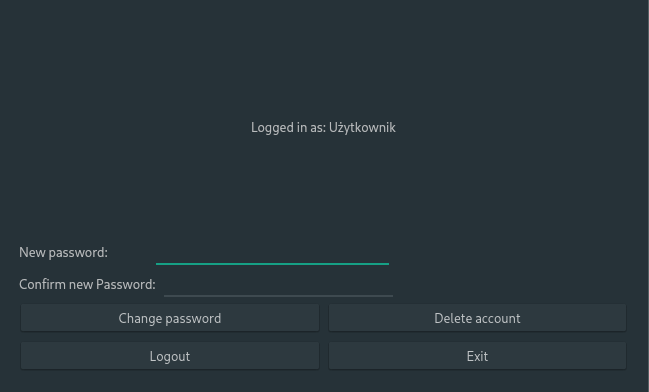
\includegraphics[width=10cm]{img/UI/user.png}
    \centering
    \caption{Panel użytkownika}
    \label{img:gui-user}
\end{figure}

\section{Szczegóły implementacji}
\subsection{Architektura systemu}
Za logikę uwierzytelniania odpowiedzialna jest klasa \textit{AuthenticationManager} oferująca metody do sprawdzenia poprawności danych, tworzenia i~usuwania kont oraz zmiany hasła. Wewnętrznie komunikuje się z klasą \textit{DatabaseAccess} będącą warstwą dostępu do użytej pozytywnej bazy danych.
Obiekty opisujące poszczególne widoki tj. \textit{LoginScreen}, \textit{RegisterScreen} oraz \textit{UserScreen} są w hierarchi poniżej klasy okna głównego -- \textit{MainWindow}. Zbierają dane przekazane przez użytkownika z~odpowiednich pól interfejsu i~tworzą odpowiednie 
zapytania do \textit{AuthenticationManager}.
Przed oddelegowaniem do procedur tworzenia konta i~zmiany hasła dane muszą być zweryfikowane jako poprawne za pomocą klasy \textit{PasswordStrengthValidator}, sprawdzającej czy dane hasło spełnia zaprogramowane zasady bezpieczeństwa.
Żeby tworzenie hasła powiodło się musi mieć następujące cechy:
\begin{itemize}
    \item Długość musi wynosić 8 lub więcej znaków
    \item Musi zawierać co najmniej jedną małą literę, jedną wielką literę, jedną cyfre oraz jeden znak specjalny
    \item Nie może być identyczne jak nazwa użytkownika (z pominięciem wielkości liter)
\end{itemize}

\begin{figure}[h]
    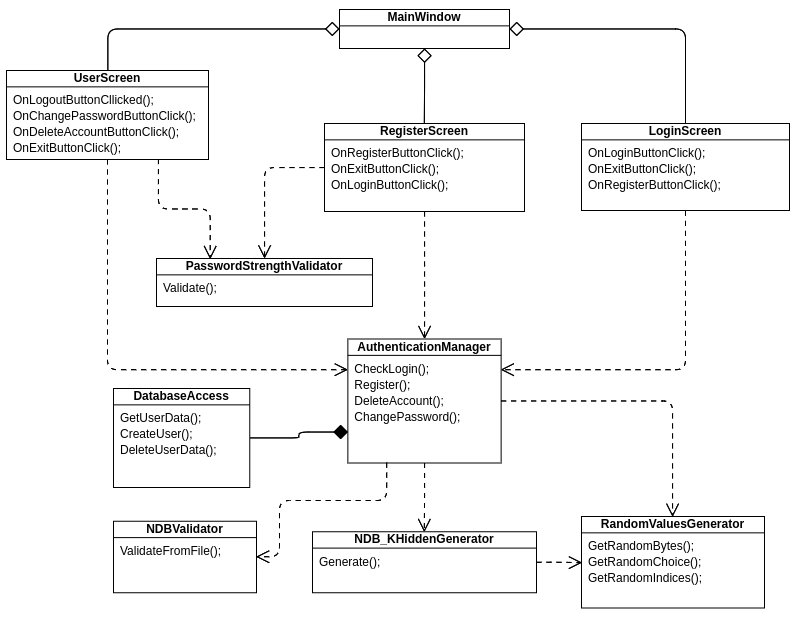
\includegraphics[width = 15.5cm]{img/diagrams/class.png}
    \centering
    \caption{Diagram klas aplikacji}
    \label{img:class}
\end{figure}



\subsection{Algorytm tworzenia użytkownika}
Jeśli dane zostały uznane jako bezpieczne z~punktu widzenia złożoności hasła, obiekty opisujące interfejs tworzą zapytanie o~stworzenie konta. Następnie \textit{AuthenticationManager} sprawdza, czy w bazie nie istnieje użytkownik
o~takiej samej nazwie -- jeśli tak, to proces kończy się porażką i~użytkownik jest o~tym informowany. W innym przypadku tworzony jest rekord $DB$. Sól jest generowana za pomocą klasy pomocniczej \textit{RandomValuesGenerator}.
Następnie tworzony jest obiekt \textit{NDB\_KHiddenGenerator} i~inicjalizowany odpowiednimi parametrami. Powstała $NDB$ jest generowana do pliku i~jej ścieżka oraz pozostałe dane umieszczane są w bazie relacyjnej.
\begin{figure}[h]
    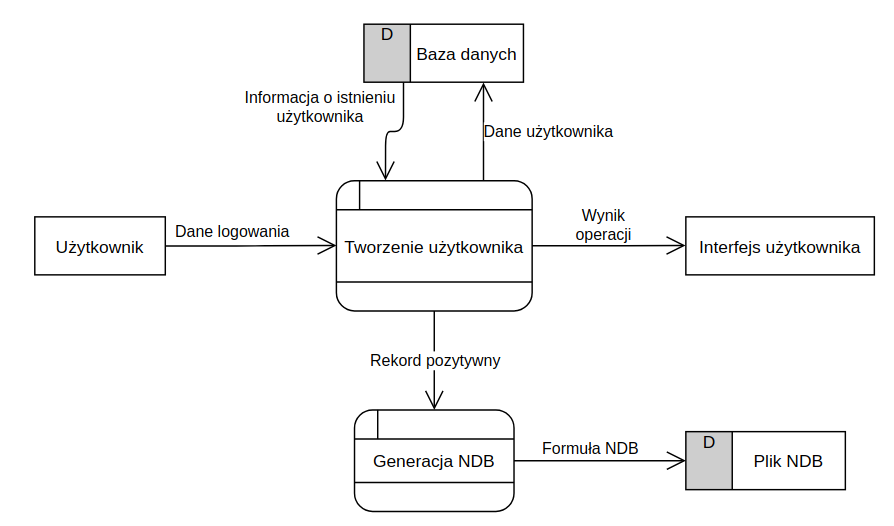
\includegraphics[width = 15.5cm]{img/diagrams/dfdregister.png}
    \centering
    \caption{Diagram przepływu danych w algorytmie tworzenia użytkownika}
    \label{img:dfd-register}
\end{figure}

\subsection{Algorytm uwierzytelniania użytkownika}
Po uzyskaniu od użytkownika loginu i~hasła dane konta są pobierane z~bazy SQLite3, jeżeli istnieją. Następnie wczytywany jest plik $NDB$ za pomocą klasy \textit{NDBValidator}, która sprawdza czy rekord zawierający skrót danego hasła
faktycznie nie pokrywa się z~żadnym rekordem negatywnym. W takim przypadku \textit{AuthenticationManager} zwraca sygnał, że użytkownik powinien mieć dostęp do danych.

\begin{figure}[h]
    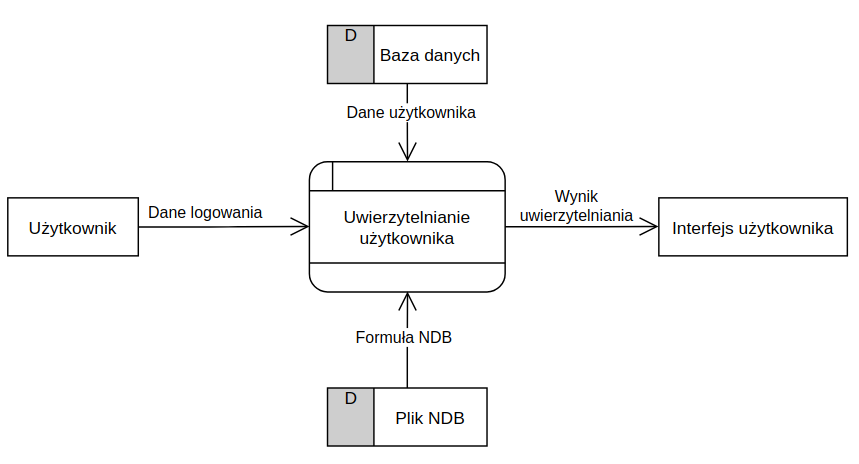
\includegraphics[width = 15.5cm]{img/diagrams/dfdlogin.png}
    \centering
    \caption{Diagram przepływu danych w algorytmie logowania}
    \label{img:dfd-login}
\end{figure}


\subsection{Algorytm zmiany hasła}
Po otrzymaniu zapytania o~zmianę hasła pobierana jest ścieżka do pliku dotychczasowej $NDB$ i~generowany jest nowy rekord $DB$ na podstawie algorytmu tworzenia użytkownika. Następnie inicjalizowany jest nowy obiekt generatora $NDB$ i~wynik jego działania zastępuje
dotychczasowe hasło w postaci negatywnej.

\begin{figure}[h]
    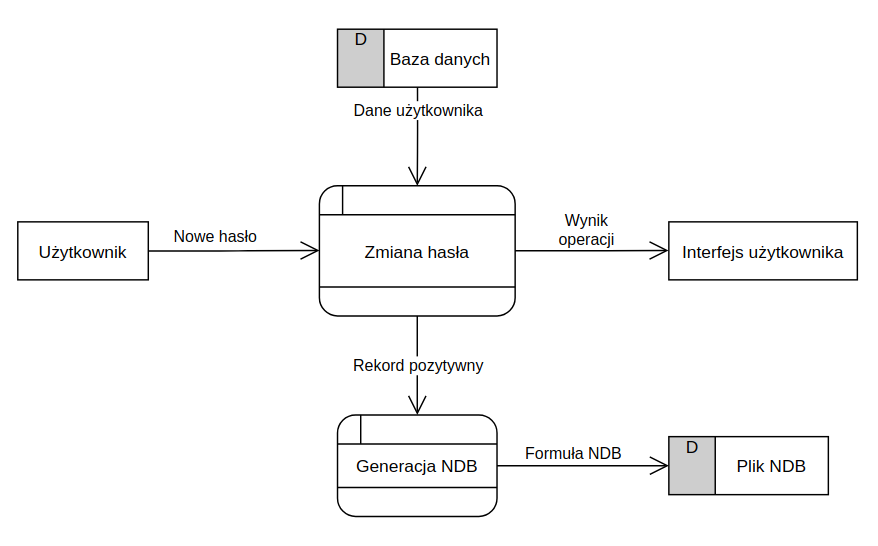
\includegraphics[width = 15.5cm]{img/diagrams/dfdchange.png}
    \centering
    \caption{Diagram przepływu danych w algorytmie zmiany hasła}
    \label{img:dfd-change}
\end{figure}

